\documentclass[xcolor=dvipsnames,aspectratio=169]{beamer}
\usecolortheme[dark,accent=cyan]{solarized}
\usepackage[utf8]{inputenc}
\usepackage{multicol}
\usepackage{url}
\usepackage{hyperref}
\usepackage{subfig}
\title{Cryptography}
\author{Gaspare Ferraro\\ ferraro@gaspa.re}
\subtitle{Hackers ahead of time}

\begin{document}

\begin{frame}[plain]
\maketitle
\begin{columns}
\column{0.5\textwidth}
	\center {
		
\includegraphics[width=0.3\textwidth]{style/qrcode.png}\\
		Visit us!
		}
\column{0.5\textwidth}
	\center{
		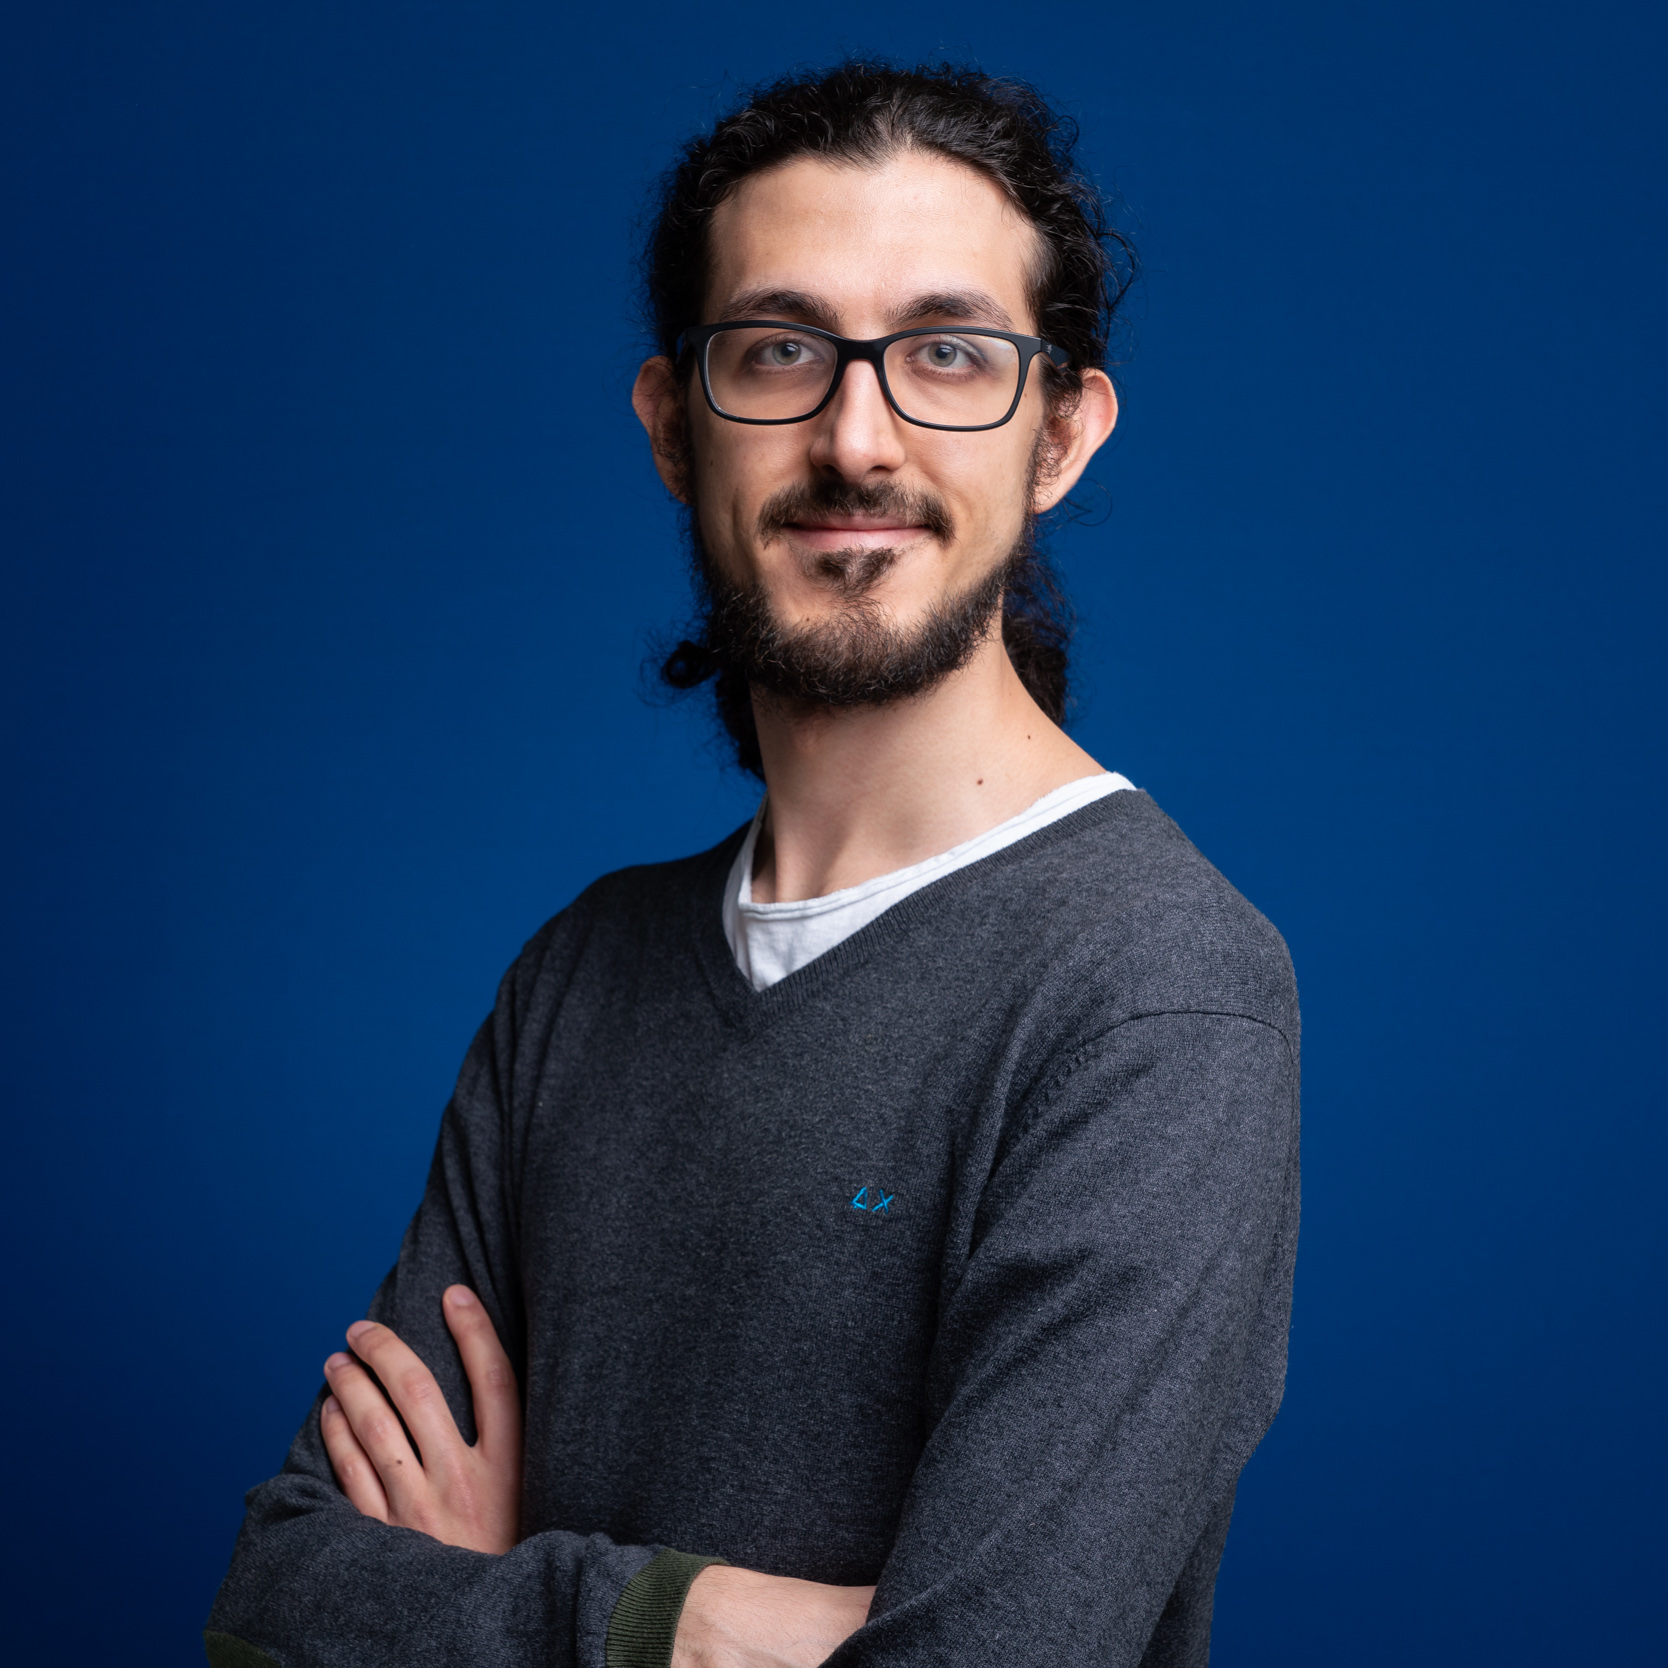
\includegraphics[width=0.3\textwidth]{style/gaspare.jpg}\\
		@GaspareG
	}
	
\end{columns}
\end{frame}

%%%%%%%%%%%%%%%%%%%%%%%%%%%%%%%%%%%%%%%%%%%%%%%%%%%%%%%%%%%%%%%%%%%%%%%%%%%%%%%
%%%%%%%%%%%%%%%%%%%%%%%%%%%%%%%%%%%%%%%%%%%%%%%%%%%%%%%%%%%%%%%%%%%%%%%%%%%%%%%

\part{Introduzione}

\begin{frame}
	\partpage
	\centering
\end{frame}

\begin{frame}{Warning!}

  \center {
    In questo incontro si fa uso della {\color{red} \textit{matematica}}! 
    
    \medskip
    
    \pause

    
\includegraphics[width=0.5\textwidth]{img/meme}
    
    \medskip
    
    \pause

    Non è sempre stato così però...
  }
  
\end{frame}

\begin{frame}{La crittografia ieri}
    
  \pause

  \begin{figure}%
    \centering
    \subfloat[Cifrario di Cesare]{{
  \centering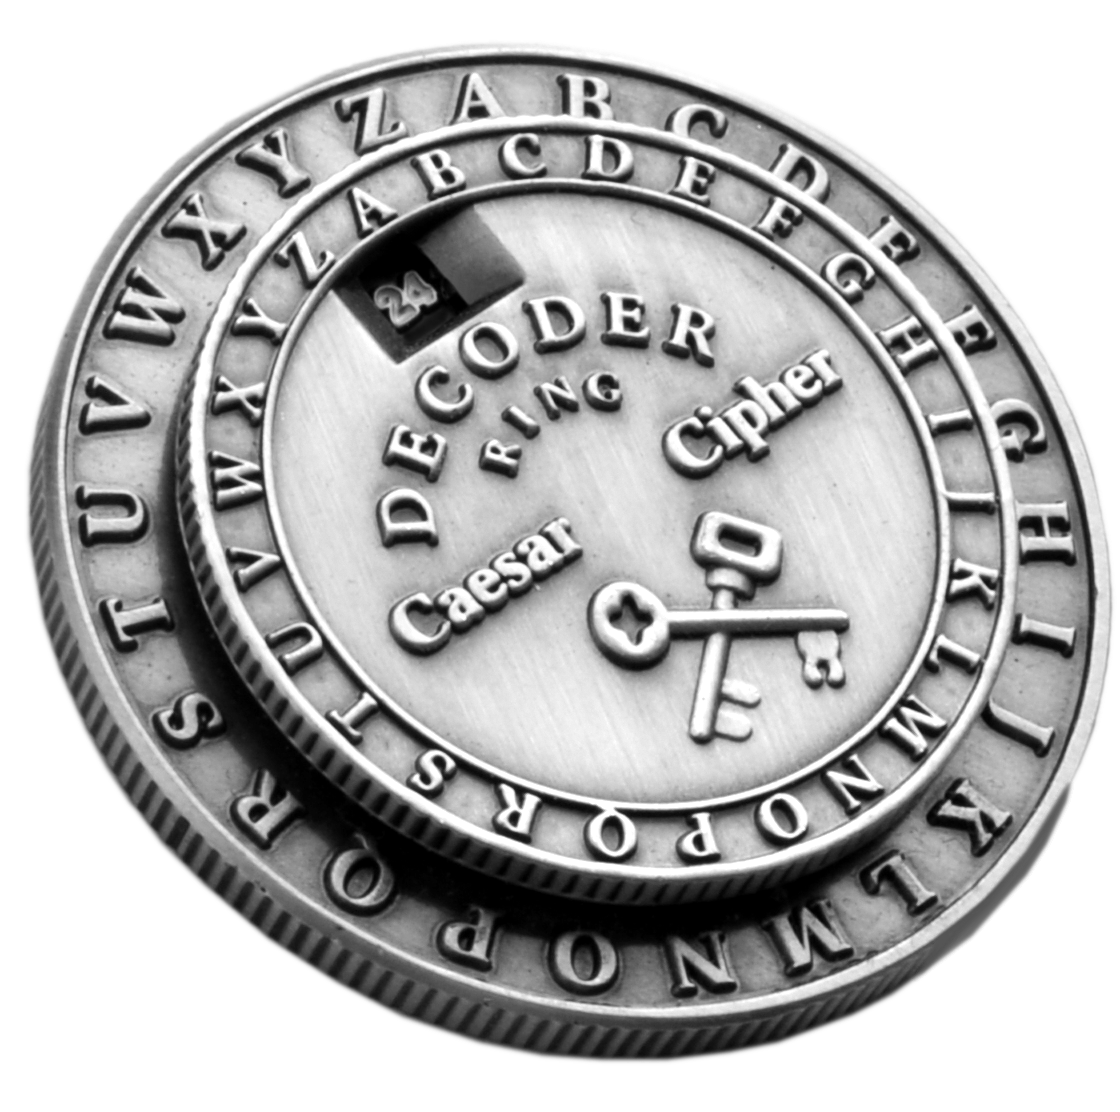
\includegraphics[width=5cm]{img/cesaer.png} }}%
  \pause
    \qquad
    \subfloat[Scitala]{{
  \centering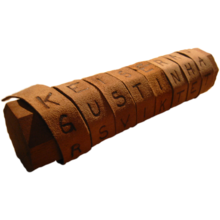
\includegraphics[width=5cm]{img/scitala.png} }}%
    %\caption{2 Figures side by side}%
    %\label{fig:example}%
  \end{figure}


\end{frame}

\begin{frame}{La crittografia oggi}
  \center {
    Le necessità, così come le risorse a disposizione, si sono evolute 
    
    ed oggi possiamo suddividere la crittografia in:
     
    \pause
    
    \medskip
    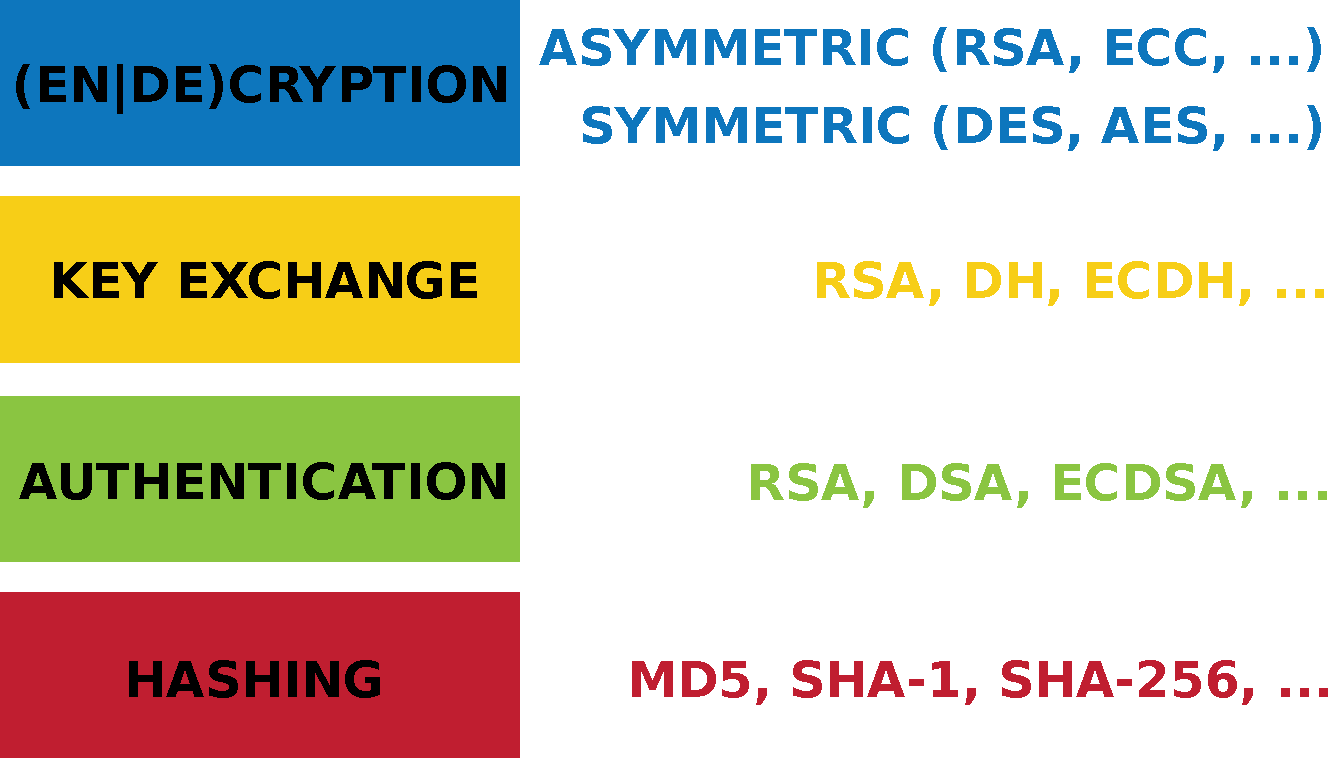
\includegraphics[width=0.6\textwidth]{crypto-section.pdf}
  }
\end{frame}
%%%%%%%%%%%%%%%%%%%%%%%%%%%%%%%%%%%%%%%%%%%%%%%%%%%%%%%%%%%%%%%%%%%%%%%%%%%%%%%
%%%%%%%%%%%%%%%%%%%%%%%%%%%%%%%%%%%%%%%%%%%%%%%%%%%%%%%%%%%%%%%%%%%%%%%%%%%%%%%

\part{Crittografia simmetrica}

\begin{frame}
	\partpage
	\centering
\end{frame}

\begin{frame}{Crittografia simmetrica}

  \pause

  I cifrari simmetrici sono quelli dove i messaggi $m$ vengono cifrati e decifrati usando una stessa chiave $k$, che deve essere nota solo ed esclusivamente alle due parti.
  
  \medskip

  \pause
  $\mathcal{C}(m, k) = c$ (funzione di cifratura)
    
  $\mathcal{D}(c, k) = m$ (funzione di decifratura)
  
  \medskip

  Ovviamente deve valere che:
  
  $\mathcal{D}(\mathcal{C}(m, k), k) = m$ (il messaggio originale non viene alterato durante lo scambio).
  
  \medskip
  \pause
  
  Per esempio nel cifrario di Cesare:
  
  $\mathcal{C}(m, k) = $ ruota in avanti di $k$ ogni singolo carattere.
  
  $\mathcal{D}(c, k) = $ ruota indietro di $k$ ogni singolo carattere.
  
\end{frame}

\begin{frame}{I principi di Shannon}

  \pause
  Come valutiamo se un cifrario è abbastanza robusto? (Dove con robustezza è intesa la sua possibilità di essere attaccato con successo). 
  
  \medskip
  \pause
  Shannon definisce due concetti chiave:
  
  \begin{itemize}
    \item Confusione: la chiave deve essere ben distribuita nel cifrato (ogni bit del cifrato dovrebbe dipendere da ogni bit della chiave).
    \item Diffusione: il messaggio deve essere ben distribuito nel cifrato (ogni bit del cifrato dovrebbe dipende da ogni bit del messaggio).
  \end{itemize}
  
  \medskip
  \pause
  
  Nel caso del cifrario di Cesare non abbiamo nessun tipo di diffusione e una bassa confusione (perchè?).
  
\end{frame}

\begin{frame}{XOR cipher}

  Consideriamo l'operazione XOR $\oplus$ (or esclusivo), valgono le seguenti proprietà:
  
  \begin{itemize}
    \item $0 \oplus 0 = 1 \oplus 1 = 0$ 
    \item $0 \oplus 1 = 0 \oplus 1 = 1$ 
    \item $x \oplus y \oplus y = x$ 
  \end{itemize}
  
  \medskip
  \pause
  
  Definiamo lo XOR cipher come:
    
  $\mathcal{C}(m, k) = m \oplus k$ 
  
  $\mathcal{D}(c, k) = c \oplus k$

  \medskip
  
  \pause

  Problema: la chiave $k$ potrebbe essere più corta del messaggio $m$.
  
  Soluzione: usiamo ripetutamente la chiave: $k^{'} = k \cdot k \cdot \ldots \cdot k$ fino a raggiungere (o superare) la lunghezza di $m$.

  \medskip
  \pause
  
  Esempio:
  
  \texttt{m = 01100011 01101001 01100001 01101111} (ciao in ASCII).\\
  \texttt{k = 01111000 01111000 01111000 01111000} (x in ascii 4 volte)\\
  \texttt{c = 00011011 00010001 00011001 00010111} (non stampabile, \texttt{GxEZFw==} in b4)
  
  
\end{frame}

\begin{frame}{Crittoanalisi statistica}

  \pause
  
  Spesso la vulnerabilità non è nell'algoritmo ma nella sua applicazione...
  
  \pause

  \medskip

  \begin{itemize}
    \item La chiave è troppo corta rispetto al messaggio
    \item La chiave viene ripetuta svariate volte per cifrare diversi messaggi
    \item I messaggi usano un dizionario mal distribuito.
    \item Conosciamo il formato del messaggio (es: \texttt{flag\{$\ldots$\}})
  \end{itemize}
  
  \medskip
  
  \pause

  In particolare parliamo di crittoanalisi statistica quando forziamo il cifrario non dal punto di vista algoritmico ma da quello statistico.
  
  \pause

  Ad esempio in italiano il $33\%$ delle lettere usate è una tra le vocali \texttt{a, e, i} mentre solo con probabilità dello $0.5\%$ si tratterà di una \texttt{z} o una \texttt{q}.


\end{frame}

\begin{frame}{Crittoanalisi statistica}
  
  \centering
  
  Strumento comodo per l'analisi statistica dei messaggi cifrati:

  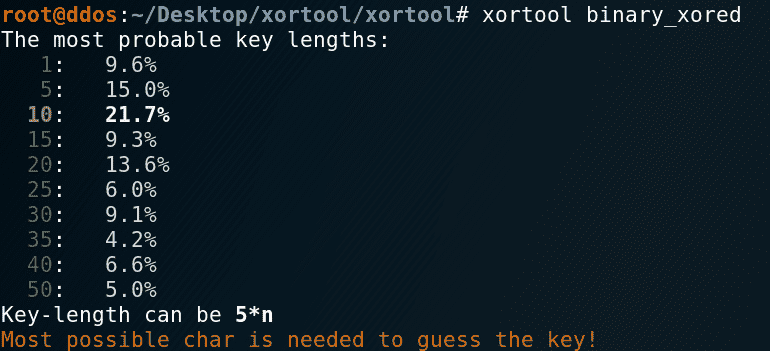
\includegraphics[width=5.5cm]{img/xortool} 

  \pause
  
  Conoscendo la parte iniziale si intravedono delle parole in chiaro:
   
  \centering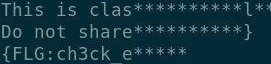
\includegraphics[width=4cm]{img/xor1} 

  Andando a tentativi si ricostruire la flag finale:
  
  
  \centering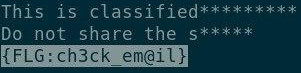
\includegraphics[width=4cm]{img/xor2} 
  
\end{frame}


\begin{frame}{One-time Pad}
  
  \pause
  
  Il problema dello XOR cipher è che cifrare usando ripetutamente la stessa chiave può far trapelare delle informazioni \textit{statistiche} sul messaggio originale.
  
  \medskip
  
  \pause
  Parliamo quindi di Cifrario di Vernam (o one-time pad) quando la lunghezza della chiave è uguale a quella del messaggio, questo cifrario è chiamato \textit{perfetto} perchè vale:
  
  \medskip
  
  $P(M = m | K = k) = P(M = m)$
  
  \medskip
  
  Ovvero la probabilità che $M$ sia un certo messaggio sapendo la chiave $K$ è uguale alla probabilità che $M$ sia un certo messaggio non sapendo la chiave (tutti i messaggi sono equiprobabili, la chiave non ci fornisce informazioni sul messaggio originale).
  
  \medskip
  
  \pause

  Bello in teoria, ma:
  
  \begin{itemize}
    \item La chiave deve essere scambiata usando un metodo sicuro (scambiarle \textit{a mano}).
    \item La chiave deve essere generata casualmente e non riusata (altrimenti è possibile un many-time pad attack).
  \end{itemize}
  
\end{frame}

\begin{frame}{DES \& AES}
  
  Data Encryption Standard (DES) e Advanced Encryption Standard (AES) si basano sul concetto della \textit{S-Box} (scatola della sostituzione).

  \pause
  
  \medskip
  
  \centering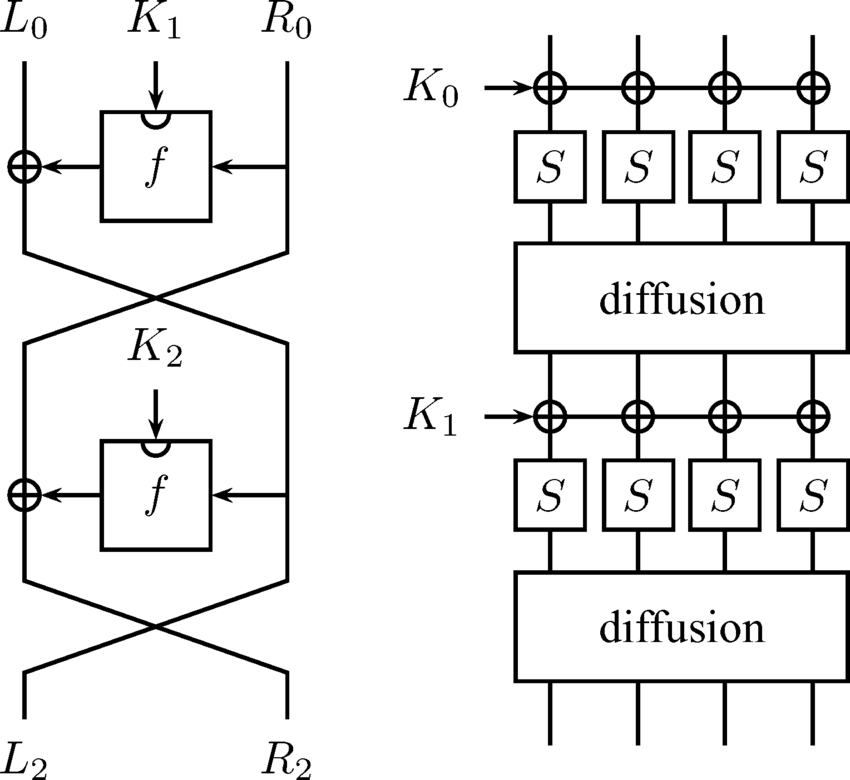
\includegraphics[width=5cm]{img/des} 
  
  \medskip

  La confusione e la diffusione vengono implementate effettuando un (elevato) numero di operazioni invertibili.
  
\end{frame}

%%%%%%%%%%%%%%%%%%%%%%%%%%%%%%%%%%%%%%%%%%%%%%%%%%%%%%%%%%%%%%%%%%%%%%%%%%%%%%%
%%%%%%%%%%%%%%%%%%%%%%%%%%%%%%%%%%%%%%%%%%%%%%%%%%%%%%%%%%%%%%%%%%%%%%%%%%%%%%%

\part{Crittografia asimmetrica}

\begin{frame}
	\partpage
	\centering
\end{frame}

\begin{frame}{Concetti base}
  La crittografia asimmetrica si basa sulle funzioni \textit{one-way trapdoor} e sulla presenza di una coppia di chiavi (chiamate chiave pubblica e chiave privata).
  
  \pause
  
  \medskip
  
  Una funzione $f$ si dice \textit{trapdoor} se: 
  \begin{itemize}
    \item Calcolare $y = f(x)$ è computazionalmente facile.
    \item Calcolare $x = f^{-1}(y)$ è computazionalmente difficile \textit{(senza nessuna informazione aggiuntiva)}.
  \end{itemize}

  \pause
  
  \smallskip
  
  Un esempio è il problema della fattorizzazione:
  \begin{itemize}
    \item $m = f(\{p, q\}) = (p * q)$ (calcolo del prodotto tra i primi $p$ e $q$).
    \item $\{p, q\} = f^{-1}(m) =\ {\color{red}??} $ (scomposizione in fattori primi di $n$).
  \end{itemize}
    
  \smallskip
  
  \pause
  
  $f(\{49171, 61843\}) = 3040882153$ (facile quanto aprire una calcolatrice).
  $f^{-1}(1841488427) = ??$ (devo provare tutti i divisori da $2$ a $\sqrt{n}$).
  
  \pause
  
  Il problema diventa banale se conosco uno dei due divisori:
  $1841488427 / 58049 = 31723$

\end{frame}

\begin{frame}{Aritmetica modulare}

Diciamo che due interi $a$ e $b$ sono congrui modulo $n$, scritto $a \equiv b$ (mod $n$), se

$(a\ \%\ n) = (b\ \%\ n)$ dove \% è il resto della divisione intera (modulo).

\medskip

\pause

Alcune proprietà matematiche:

\pause

\begin{itemize}
  \item $a + k\equiv b + k$ (mod $n$), invariante per addizione.
  \item $k*a \equiv k*b$ (mod $n$), invariante per moltiplicazione.
  \item $a^k \equiv b^k$ (mod $n$), invariante per potenza.\pause
  \item $\sqrt{a} \equiv b$ (mod $n$) se $a \equiv b^2$ (mod $n$), radice quadrata.
  \item $a^{-1} \equiv b$ (mod $n$) se $ab \equiv 1$ (mod $n$), inverso moltiplicativo.
  \item ...
\end{itemize}

\end{frame}

\begin{frame}{RSA pt.1}

\pause

L'algoritmo di cifratura asimmetrica più famoso è l'RSA (da {\color{red}R}ivest {\color{red}S}hamir {\color{red}A}dleman) che si basa sul problema della fattorizzazione e sull'aritmetica modulare.

\pause

\smallskip

Il funzionamento di base è:\pause

\begin{itemize}
  \item Si scelgono due numeri primi a caso $p$ e $q$ (in modo \textit{sicuro}).\pause
  \item Si calcola il prodotto $n = p*q$ (che sarà il nostro modulo).\pause
  \item Si calcola il toziente $\phi(n) = (p-1)*(q-1)$ (il numero dei coprimi con $n$).\pause
  \item Si sceglie a caso un numero $e$, coprimo e minore di $\phi(n)$.\pause
  \item Si calcola il numero $d$ come inverso moltiplicativo di $e$, ovvero $ed \equiv 1$ (mod $\phi(n)$).
\end{itemize}

\medskip

\pause

Chiamiamo quindi:

\pause

$k_{pub} = (n, e)$ la chiave pubblica che distribuiamo.

\pause

$k_{priv} = (n, d)$ la chiave privata che teniamo segreta.

\end{frame}

\begin{frame}{RSA pt.2}

Una volta calcolata la chiave pubblica e quella privata possiamo cifrare e decifrare i messaggi in questo modo:

\pause
\medskip

$\mathcal{C}(m, k_{pub}) = m^{e} $ (mod $n$) \pause
  
$\mathcal{D}(c, k_{priv}) = c^{d} $ (mod $n$)

\medskip

\pause

Si ma perchè funziona?

\medskip

\pause

Dal teorema di Eulero sappiamo che $m^{\phi(n)} \equiv 1 $ (mod $n$).

I valori $e$ e $d$ sono calcolati in modo che $ed \equiv 1$ (mod $\phi(n)$).

\medskip

$\mathcal{D}(\mathcal{C}(m, k), k) = m^{ed} = m^{\phi(n)*t + 1} = m^{\phi(n)^{t}} * m = 1 * m = m$

\end{frame}

\begin{frame}{Un esempio per capire}
  
\pause

  Scegliamo i sequenti parametri:
  
  \begin{itemize}
    \item $p = 13$ e $q = 23$
    \item $n = p*q = 299$
    \item $\phi(n) = (13-1)*(23-1) = 264$
    \item $e = 7$, $\gcd(264, 7) = 1$
    \item $d = 151$, $7*151 \equiv 1 $ (mod $264$)
  \end{itemize}
  
  \smallskip
  
\pause

  Quindi $k_{pub} = (299, 7)$ e $k_{priv} = (299, 151)$. Vogliamo cifrare $m = 42$.
  
\pause

  \medskip
  
  $\mathcal{C}(m, k_{pub}) = m^{e} = 42^7 = 230539333248 = 107$ (mod $299$) 
 
 \pause
  
  $\mathcal{D}(c, k_{priv}) = c^{d} = 107^{151} = 2743956545...948643 = 42 $ (mod $299$)

\end{frame}

\begin{frame}{(Non tanto) a caso}

\pause

"Si scelgono due numeri primi \textit{a caso} $p$ e $q$ (in modo \textit{sicuro})"

\begin{itemize}
  \item Scegliere $p$ e $q$ di almeno $1024$ bit.
  \item Scegliere $p$ e $q$ non troppo vicini tra loro.
  \item Non riusare uno dei primi per altri moduli.
\end{itemize}

\smallskip
\pause
Con la potenza di calcolo attuale è possibile fattorizzare semiprimi fino a (circa) $768$ bit, i moduli più grandi sono (per ora) resistenti agli attacchi bruteforce.

\smallskip
\pause
Se $p$ e $q$ sono vicini allora abbiamo che $n \simeq p^2 \simeq q^2$ e quindi anche $\sqrt{n}$ sarà vicino ai primi. Basterà quindi un attacco bruteforce che cerca i fattori vicino alla radice quadrata.

\smallskip
\pause

Se $n_1 = p*q^{'}$ e $n_2 = p*q^{''}$ allora $p = \gcd(n_1, n_2)$.

\end{frame}

%%%%%%%%%%%%%%%%%%%%%%%%%%%%%%%%%%%%%%%%%%%%%%%%%%%%%%%%%%%%%%%%%%%%%%%%%%%%%%%
%%%%%%%%%%%%%%%%%%%%%%%%%%%%%%%%%%%%%%%%%%%%%%%%%%%%%%%%%%%%%%%%%%%%%%%%%%%%%%%

\part{Hashing}

\begin{frame}
	\partpage
	\centering
\end{frame}

\begin{frame}{Creare confusione}

\pause

Chiamiamo hash una funzione $f$ \textit{non invertibile} che associa una stringa ad una stringa di dimensione fissata. Con le seguenti proprietà:

\pause

\begin{itemize}
  \item Resistenza alla preimmagine: dato un hash $h$ è difficile trovare $m$ tale che $f(m) = h$.
  \item Resistenza alla seconda preimmagine: dato $m_1$ è difficile trovare $m_2$ tale che $f(m_1) = f(m_2)$.
  \item Resistenza alle collisioni: è difficile trovare coppie $(m_1, m_2)$ tali che $f(m_1) = f(m_2)$.
\end{itemize}

\pause

Utilizzi pratici:

\begin{itemize}
  \item Salvataggio delle password (hashate invece che in chiaro).
  \item Creazione di hashtable (struttura dati ad accesso diretto).
  \item Controllo di integrità (\textit{md5sum}, \textit{sha1sum}).
  \item Firma digitale (sull'hash invece che sul documento).
\end{itemize}

\end{frame}

\begin{frame}{MD5}
  
    \pause
  Inventato da Rivest nel 1991, divenne la funzione di hash standard fino al 2004-2006.
  Viene utilizzata ancora adesso per il controllo di integrità.
    
    \pause
  \medskip
  
  \centering
  {
  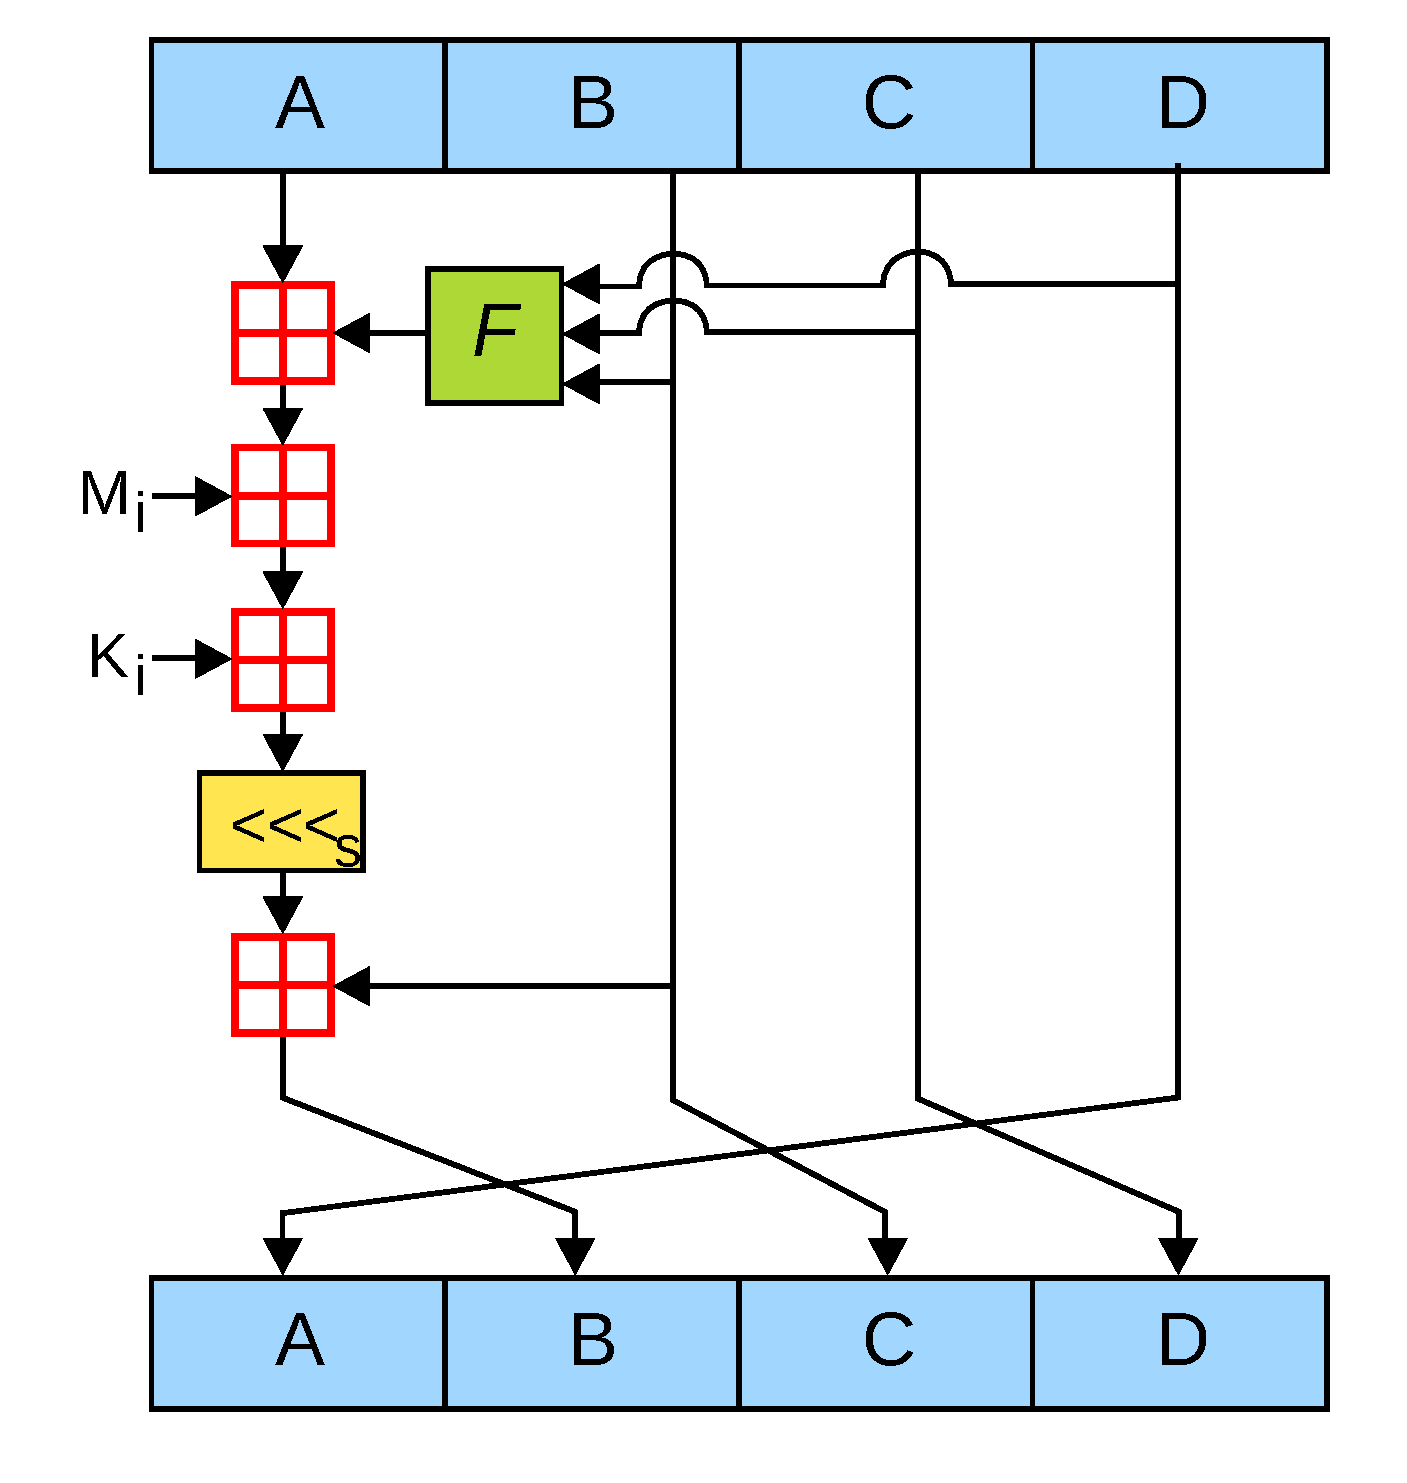
\includegraphics[width=3.8cm]{img/md5}
  }
  
    \pause
  md5("password") = \texttt{5F4DCC3B5AA765D61D8327DEB882CF99}
  
    \pause
  md5("passwore") = \texttt{A826176C6495C5116189DB91770E20CE}
  
\end{frame}

\begin{frame}{Proof of Work}
    \pause

    Spesso, come sistema di protezione per attacchi DOS o per altri motivi, ci viene chiesto di reversare (completamente o parzialmente) un hash.
    
    \pause \medskip
        
    L'accesso ad una risorsa ci verrà fornito solo dopo aver dimostrato (\textit{Proof of Work}) la risoluzione ad un problema.
    Nel caso dell'hashing questa operazione viene chiamata hashcash (ed è alla base del mining delle criptovalute).
    
    \medskip
    
    \pause

    Esempio (VolgaCtf2017):
    
    \texttt{Solve a puzzle: find an x such that 26 last bits of SHA1(x) are set, len(x)==29 and x[:24]=='58a5a7950d2ec81fae5c1c74'}
    
\end{frame}

\begin{frame}{Trovare le collisioni pt.1}

    Come trovo una collisione / preimmagine?
    
    \pause

    \begin{itemize}
      \item Database online (es. crackstation.net), immediato ma non completo.
      \item Bruteforce (es. John The Ripper, HashCat), lento ma completo.
    \end{itemize}
    
    \medskip
    \pause
    
    Quanti tentativi dovrò fare per reversare un hash?
    
    \pause
    \medskip
    
    Paradosso dei compleanni: 
    
    se la funzione hash restituisce un output da $n$ bit ($m = 2^n$ possibili hash) si avrà una collisione al 50\% di probabilità dopo $2^{(n/2)}$ tentativi ($sqrt(m)$).
    
\end{frame}

\begin{frame}{Trovare le collisioni pt.2}

    John The Ripper
    
    \medskip
    
    \centering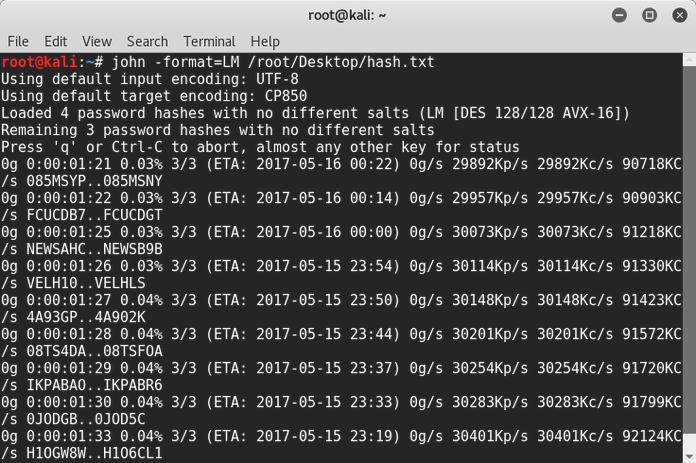
\includegraphics[width=8cm]{img/john}
    
\end{frame}
    
\begin{frame}{Trovare le collisioni pt.3}

    Hashcat
    
    \medskip
    
    \centering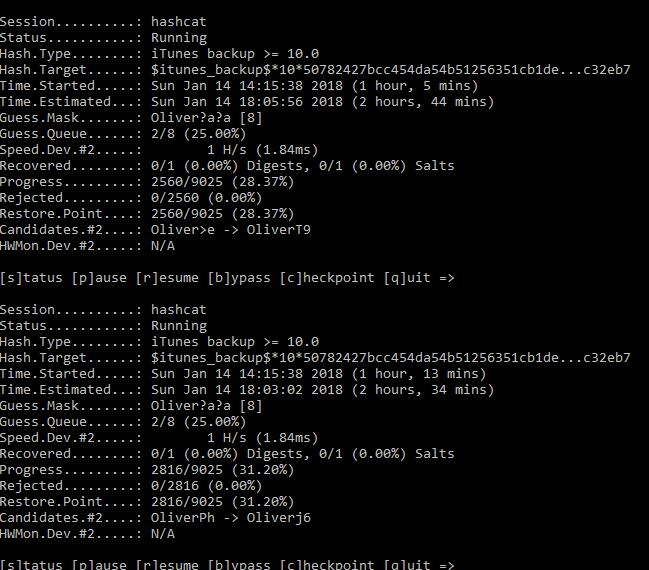
\includegraphics[width=8cm]{img/hashcat}
    
\end{frame}
    
\begin{frame}{Basta un poco di sale...}
  
  ...e la password non va giù.
  
  \medskip

  \pause
  Abbiamo parlato di come \textit{non salvare le password in chiaro} bensì salvare il loro hash.
  
  \medskip
  \pause

  Problema: 
  
  Se più persone usano le stessa password (tipico: \textit{qwerty}, \textit{123456}, ..., vedi SAW17/18) avrò hash duplicati nel database.
  
  \medskip
  \pause
  Soluzione: 
  
  Salvare f(password + salt) invece che f(password), dove \textit{salt} è una stringa casuale generata per persona (possibilmente memorizzata in un luogo separato ai dati di login).
  
\end{frame}

\begin{frame}{Un (pessimo) esempio...}
    \pause

  \begin{figure}%
    \centering
    \subfloat{{
  \centering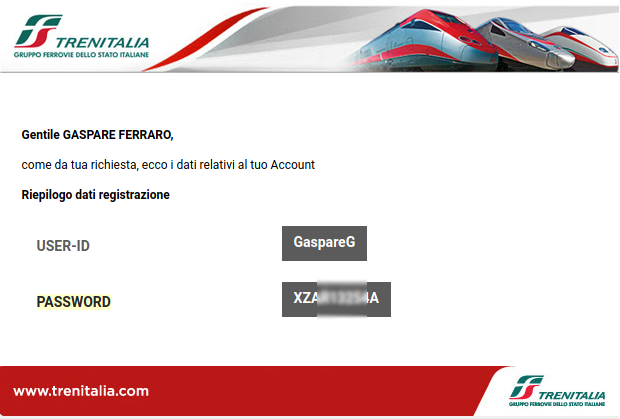
\includegraphics[width=7cm]{img/trenitalia2} }}%
  \pause
    \qquad
    \subfloat{{
  \centering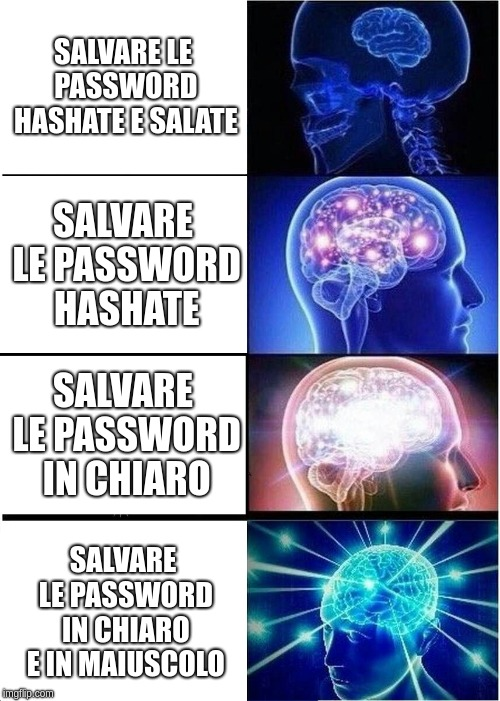
\includegraphics[width=5cm]{img/trenitalia} }}%
    %\caption{2 Figures side by side}%
    %\label{fig:example}%
  \end{figure}

\end{frame}
%%%%%%%%%%%%%%%%%%%%%%%%%%%%%%%%%%%%%%%%%%%%%%%%%%%%%%%%%%%%%%%%%%%%%%%%%%%%%%%
%%%%%%%%%%%%%%%%%%%%%%%%%%%%%%%%%%%%%%%%%%%%%%%%%%%%%%%%%%%%%%%%%%%%%%%%%%%%%%%
\begin{frame}{Fine}

\end{frame}
%%%%%%%%%%%%%%%%%%%%%%%%%%%%%%%%%%%%%%%%%%%%%%%%%%%%%%%%%%%%%%%%%%%%%%%%%%%%%%%
%%%%%%%%%%%%%%%%%%%%%%%%%%%%%%%%%%%%%%%%%%%%%%%%%%%%%%%%%%%%%%%%%%%%%%%%%%%%%%%

\end{document}
